% Fuentes que no vi:
% https://www.youtube.com/@AuxiRolando
\documentclass[a4paper]{article}
\usepackage[margin=1.5cm]{geometry}
%\documentclass[11pt]{article}
%\usepackage[paperwidth=9cm,paperheight=60cm,margin=0.4cm]{geometry}
\usepackage{multicol}
\usepackage{enumitem}
\usepackage{graphicx}
%Links
\usepackage[colorlinks = true,
            linkcolor = blue,
            urlcolor  = blue,
            citecolor = blue,
            anchorcolor = blue]{hyperref}
%Simbolos matemáticos
\usepackage{amsmath}
\usepackage{amssymb}
%Manejo de argumentos en los comandos
\usepackage{xparse}
%Enumeracion
\usepackage{enumitem}
%Páginas sin numeración
\pagestyle{empty}
%Interlineado
\renewcommand{\baselinestretch}{1.5}
%Arreglar comillas
\usepackage [autostyle]{csquotes}
\MakeOuterQuote{"}
%Macros
\newcommand{\Item}{\item[\stepcounter{enumii}$\blacktriangleright$\textbf{(\alph{enumii})}]} %Negrita en algunos items
\newcommand{\answer}{\item[**]}
\newcommand{\exercise}{\item}
%Logic macros
\newcommand{\then}{\to}
\newcommand{\eq}{\leftrightarrow}
\newcommand{\xor}{\veebar}
\newcommand{\nor}{\downarrow}
\newcommand{\nimply}{\nrightarrow}
\newcommand{\nand}{\uparrow}
\newcommand{\Then}{\Rightarrow}
\newcommand{\Eq}{\Leftrightarrow}
% Command to format each premise or reasoned proposition
\NewDocumentCommand{\FormatItem}{m}{%
    #1 \\[-4pt]
}
% Define the \Reasoning command
\NewDocumentCommand{\Reasoning}{>{\SplitList{;}}m m}{%
    \begin{minipage}[t]{\linewidth}
    \ProcessList{#1}{\FormatItem} % Process each premise
    \\[-24pt] \hspace{-.5cm}\rule[.5pt]{2.2cm}{.5pt}\\[-8pt]
    #2 \\[-8pt]% This is the conclusion
    \end{minipage}%
}
% Define the \DReasoning command
\NewDocumentCommand{\DReasoning}{>{\SplitList{;}}m >{\SplitList{;}}m m}{%
    \begin{minipage}[t]{\linewidth}
    \ProcessList{#1}{\FormatItem} % Process each premise
    \\[-24pt] \hspace{-.5cm}\rule[.5pt]{3cm}{.5pt}\\[-8pt]
    \ProcessList{#2}{\FormatItem} % Process each reasoned proposition
    \\[-24pt] \hspace{-.5cm}\rule[.5pt]{3cm}{.5pt}\\[-8pt]
    #3 \\[-8pt]% This is the conclusion
    \end{minipage}%
}
\begin{document}
\noindent \hrulefill 
\vspace{-7pt}
\begin{center} 
	\textbf{ Práctica 1: Lógica proposicional y de primer orden } \\
	Comisión: Rodrigo Cossio-Pérez y Leonardo Lattenero
\end{center}
\vspace{-10pt}
\hrulefill \\
\phantom{~} \\
\textbf{EJERCICIOS JR.}
\begin{enumerate}
	\exercise Reconocer las funciones del lenguaje e indicar qué casos son proposiciones. Si son proposiciones, indicar su valor de verdad.
	\begin{multicols}{2}
	\begin{enumerate} [label=(\alph*)]
		\item Hoy es martes 
		\item ¡Auch!
		\item Fuí a visitar las playas de la costa de Buenos Aires 
		\item Vaya a visitar las playas de la costa de Buenos Aires
		\item ¿Venís hoy a clase?
		\item 5 es múltiplo de 2 
		\item Si estudiás continuamente, siempre vas a aprender cosas nuevas 
		\item $x=6$ y $x+4=10$ 
		\item $x+4$ 
		\item $x^2-4$ no tiene raíces reales 
	\end{enumerate}
	\end{multicols}
	\exercise Simbolizar las siguientes proposiciones, indicar el diccionario de lenguaje cuando sea necesario y cuando amerite hallar una proposición equivalente considerando las propiedades y definiciones de los operadores.
	\begin{multicols}{2}
	\begin{enumerate} [label=(\alph*)]
		\item La manzana es una fruta y la lechuga una verdura. 
		\item No está lloviendo. 
		\item Si estás en la estación Bernal, estás cerca de la UNQ 
		\item No es buen deportista pero sus notas son excelentes.
		\item El caballo está galopando, o se detuvo y relinchó.
		\item En la UNQ hay wi-fi si y sólo si hay luz.
		\item Una de dos: o mañana lloverá o estará soleado. 
		\item La materia se aprueba promocionando los parciales, aprobando el final o dando exitosamente el exámen libre. 
		\item El pan no levará si le ponés mucha sal. Tampoco levará si lo dejás en un lugar frío. 
		\item Si te tomás el 324 te deja cerca de la UNQ, si te tomás el 65 no. 
	\end{enumerate}
	\end{multicols}
	\exercise Determinar si las siguientes proposiciones son tautologías, contradicciones o contingencias mediante la realización de su tabla de verdad. 
	\begin{multicols}{2}
	\begin{enumerate} [label=(\alph*)]
		\item $(\neg p \lor  q) \land  \neg q$
		\item $p \land  \neg p$
		\item $p \land  F_0 \lor  q$
		\item $(p \then  q) \then  r$
		\item $p \eq (q \xor  r)$
		\item $(p \nand q) \nor r$
		\item $((\neg p \lor q) \then (r \lor p)) \lor (p \then q)$
	\end{enumerate}
	\end{multicols}
	\exercise Averiguar si las siguientes proposiciones son equivalentes mediante tablas de verdad y/o reglas de equivalencia.  Dar un ejemplo en lenguaje natural que lo evidencie. Nota: no siempre el mismo método.
	\begin{multicols}{2}
	\begin{enumerate} [label=(\alph*)]
		\item $\neg (\neg p) \Eq  p$
		\item $p\then q \Eq \neg q\then \neg p$
		\item $p\then q \Eq \neg p\then \neg q$
		\item $p \land  (p \lor  q) \Eq  p$
		\item $p\then q	\Eq (p \land  \neg q)\then F_0$
		\item $(p\land q)\then r \Eq p\then (q\then r) $
		\item $p\lor q \then  r	\Eq (p\then r) \land  (q\then r)$
	\end{enumerate}
	\end{multicols}
	\exercise Simplificar las siguientes expresiones
	\begin{multicols}{2}
	\begin{enumerate} [label=(\alph*)]
		\item $\neg ((p \land \neg q)\then p) \lor q$
		\item $(\neg q \then \neg p) \land \neg (\neg p \then \neg q)$
		\item $(\neg q \lor p) \lor (p \land \neg q)$
		\item ($p \land ( p \then q)) \then q$
		\item $\neg ((\neg p \land q) \then p) \lor q$
		\item $(\neg p \then q) \land \neg (q \then \neg p)$
	\end{enumerate}
	\end{multicols}
	\exercise Escribir en forma normal disyuntiva (DNF) y en forma normal conjuntiva (CNF) las siguientes proposiciones.
	\begin{multicols}{2}
	\begin{enumerate} [label=(\alph*)]
		\item $p\xor q$
		\item $\neg (p \nand q) \lor \neg p$
		\item $p\then  (q\land r)$
	\end{enumerate}
	\end{multicols}
	\exercise Verificar mediante una tabla de verdad si las siguientes proposiciones son reglas de inferencia. Dar un ejemplo en lenguaje natural que lo evidencie.
	\begin{multicols}{2}
	\begin{enumerate} [label=(\alph*)]
		\item $p \land q \Then p$
		\item $p\lor q \Then  q$
		\item $p \land  T_0 \Then  q$
		\item $(\neg p \land q) \Then (\neg p \lor q)$
		\item $(p\eq q) \Then  (p\then q)$
		\item $((p \eq q) \land r ) \Then \neg (q \land r)$
	\end{enumerate}
	\end{multicols}
	\exercise Sin utilizar las tablas de verdad, demostrar si los siguientes razonamientos son válidos o no. 
	\begin{multicols}{3}
	\begin{enumerate} [label=(\alph*)]
		\item \Reasoning{$\neg p\then p$}{$p$}
		\item \Reasoning{$p\then q$ ; $\neg q$}{$\neg p$}
		\item \Reasoning{$p\then q$ ; $q\then r$ ; $p$}{$r$}
		\item \Reasoning{$\neg p$}{$\neg (p\land q)$}
		\item \Reasoning{$p\then r$ ; $q\then r$ ; $r\then s\land t$ ; $p\lor q$}{$s$}
		\item \Reasoning{$p\then q$ ; $q\land r\then s$}{$p\land r\then  s$}
		\item \Reasoning{$p\then  q$ ; $q\eq r$ ; $\neg r$}{$\neg p$}
		\item \Reasoning{$p \then q$ ; $p \lor s$ ; $\neg q$}{$s$}
	\end{enumerate}
  \end{multicols}
	\exercise Averiguar si los siguientes razonamientos son válidos y evaluar su solidez.
	\begin{enumerate} [label=(\alph*)]
		\item Por el pronóstico semanal, sabemos que si es martes, llueve y hace frío. Sabemos que es martes. Demostrar que hace frío.
		\item El ladrón tenía llave de la puerta o entró por la ventana. Si entró por la ventana, pisoteó las macetas. Las macetas no están pisoteadas. Por lo tanto, el ladrón tenía llave de la puerta.
		\item El producto de dos enteros impares es impar
		\item La suma de dos números naturales pares es un número natural impar
		\item Si el cuadrado de un número entero es impar, dicho número es impar. 
		\item Si un número entero es múltiplo de 6, entonces dicho número es múltiplo de 2 y de 3.
		\item Si un número entero es menor que otro, el primer número es menor o igual que el sucesor del segundo
		\item Si se cumple que $x^2-x-6>0$, entonces se cumple que $|x| > 1$.
		\item Si $|x| = |y|$, entonces  $y=x$ o $y=-x$.
		\item Si $a.b = 0$, la recta $y=mx+b$ pasa por $P(0,0)$ o bien la recta $y=ax+3$ es horizontal.
	\end{enumerate}
	\exercise Simbolizar las siguientes proposiciones, indicando el diccionario de lenguaje y el conjunto universal. Cuando se indique, negar la proposición.
	\begin{enumerate} [label=(\alph*)]
		\item Alguien canta o toca la guitarra. (Adicionalmente, negar esta expresión) 
		\item Todos los números naturales son pares o negativos. (Adicionalmente, negar esta expresión) 
		\item Si un automóvil es cómodo, entonces es caro
		\item Hay gente que cuando tiene frío toma mate, y cuando no lo tiene no
		\item Ningún pájaro es un anfibio. Si un animal no es un anfibio, tampoco será un pez. Por lo tanto, ningun pájaro es pez.
	\end{enumerate}
	\exercise Indicar el valor de verdad de las siguientes proposiciones cuantificadas. 
	\begin{enumerate} [label=(\alph*)]
		\item $\exists x: P(x)$:\textit{"Según el pronóstico semanal, el día x llueve"} con $U = \{$Lunes, Martes, Miércoles, Jueves, Viernes, Sábado, Domingo$\}$
		\item $\forall x \in U: x^2 < 26$, con $U=\{1,3,5\}$
		\item $\exists x \in U: x^2 < 26$, con $U=\{1,3,5\}$
		\item $\forall x \in \mathbb{N}: x^2 -9 =0$
		\item $\forall x \in \mathbb{R}: x+3 < 6$
		\item $\exists x \in \mathbb{R}: x^2 =1$ 
		\item Dado $U = \mathbb{N}$, $\left(\forall x: x < 5\right) \lor \left( \exists x: x^2 = 4 \right)$ 
		\item $\forall x \exists y:  x < y$, donde $x$ e $y$ pertenecen al conjunto $\{1,2,3\}$.
	\end{enumerate}
	\exercise Averiguar si los siguientes razonamientos son válidos y, en el caso de que tengan un contexto, evaluar su solidez.
	\begin{multicols}{2}
	\begin{enumerate} [label=(\alph*)]
		\item Dada la variable $x$ y la constante $a$, se plantea: \\ \Reasoning{$\forall x: P(x)\then  Q(x) \land  R(x)$; $P(a)$}{$\exists x: R(x)$}
		\item \Reasoning{$Q(a) \then R(a)$; $Q(a) \then \neg R(a)$}{$\exists x: \neg Q(x)$} 
		\item Considerando $U=\{3,4,6\}$ y los predicados $A(x):$\textit{"$x$ es entero"}, $B(x):$\textit{"$x$ es par"} y $C(x):$\textit{"$x$ es múltiplo de 4"} se plantea: \\ \Reasoning{$\exists x: A(x) \then \neg B(x)$; $C(6) \lor B(6)$; $\neg C(6)$}{$\exists x: \neg A(x)$} 
		\item \Reasoning{$\neg \forall x: P(x) \then  Q(x)$}{$\exists x: P(x)$}
		\item \Reasoning{$\neg \exists x: \neg P(x) \land  \neg Q(x)$; $\neg P(a)$}{$Q(a)$}
		\item Todos los hombres son mortales. Sócrates es un hombre. Por lo tanto, Sócrates es mortal.
		\item Hay productos tienen buen precio o buena calidad. Todos los productos de buena calidad son resistentes. Entonces, hay productos que tienen buen precio o que son resistentes. 
		\item Todos los dulces contienen carbohidratos. Existen comidas sin carbohidratos que tienen proteínas. Por lo tanto, todas las comidas tienen carbohidratos o proteinas.
	\end{enumerate}
	\end{multicols}
\end{enumerate}
\textbf{EJERCICIOS SR.}
\begin{enumerate}[resume]
	\exercise Reconocer las funciones del lenguaje e indicar qué casos son proposiciones. Si son proposiciones, indicar su valor de verdad.
	\begin{multicols}{2}
	\begin{enumerate} [label=(\alph*)]
		\item Tal vez llueve
		\item ¿Está lloviendo?
		\item Dadas las rectas $R_1: y=x+1$ y $R_2: y=-x+7$, $R_1 \perp R_2$.
		\item $ [ 0, \infty )$
		\item Gracias
		\item Me parece que sí 
		\item ¡No me digas!
		\item $x=9$ y $2 < x < 7$
		\item En las aulas de la UNQ
		\item $2 < x < 7$ (donde $x$ no está definido)
		\item Si tan solo me hubiese acordado de regar el potus…
		\item A caballo regalado no se le miran los dientes 
	\end{enumerate}
	\end{multicols}
	\exercise Simbolizar las siguientes proposiciones, indicar el diccionario de lenguaje cuando sea necesario y cuando amerite hallar una proposición equivalente considerando las propiedades y definiciones de los operadores.
	\begin{multicols}{2}
	\begin{enumerate} [label=(\alph*)]
		\item Luis es feliz, si escribe poemas.
		\item No es cierto que estudiamos y no aprobamos.
		\item No me gusta la pizza ni las empanadas. 
		\item Hoy no es jueves, ya que ayer no fue miércoles.
		\item Si llueve traigo el impermeable y las botas. 
		\item Si has amado sabés lo que se siente amar, sino no. 
		\item El anciano ingresó a la cabaña y tomo asiento, o permaneció afuera; si y solo si regresó de viaje.
		\item Caminamos sin prisa pero sin pausa. 
		\item Python es un lenguaje de programación interpretado, de propósito general y de alto nivel, por lo tanto resulta útil para procesar datos o automatizar tareas simples. 
		\item Ir rápido equivale a ir despacio pero sin pausas. 
		\item O termino las tareas en la semana, con lo que tendría el fin de semana libre, o las termino durante el fin de semana, con lo que tendría que abastecerme de café o mate.  
		\item Para aprobar, basta dedicar tiempo y atención a la materia.  
		\item Calavera no chilla y piola se la banca.
		\item Vine en tren y suspendieron el servicio, así que tengo que volver en colectivo o caminando.
		\item En un juego son importantes las mecánicas y la historia. Las mecánicas mantienen a la persona jugadora activa. La historia la mantiene interesada. 
		\item Decir que los fantasmas se ponen azules cuando el pacman come la fruta, es lo mismo que decir que los fantasmas están azules o el pacman no se comió la fruta. 
	\end{enumerate}
	\end{multicols}
	\exercise Determinar si las siguientes proposiciones son tautologías, contradicciones o contingencias mediante la realización de su tabla de verdad. 
	\begin{multicols}{2}
	\begin{enumerate} [label=(\alph*)]
		\item $p \xor  (\neg q \xor  r)$
		\item $p \land  q \lor  r$
		\item $p \nimply (q \land  r)$
		\item $(T_0 \nor q) \nimply r$
		\item $(\neg p \eq q) \land \neg (q \then \neg p)$
		\item $((p \land \neg q) \then \neg r) \lor (p \xor q)$
		\item $\neg ((r \then p) \land (\neg q \lor p)) \land ( p \land (p \then r))$
		\item $\neg ((\neg p \land q) \then p ) \lor q$
	\end{enumerate}
	\end{multicols}
	\exercise Averiguar si las siguientes proposiciones son equivalentes mediante tablas de verdad y/o reglas de equivalencia.  Dar un ejemplo en lenguaje natural que lo evidencie. Nota: no siempre el mismo método.
	\begin{multicols}{2}
	\begin{enumerate} [label=(\alph*)]
		\item $\neg p\then p \Eq p$
		\item $\neg p\lor \neg q \Eq (p\land q)$
		\item $(p \land \neg q) \Eq (\neg p \lor q)$
		\item $(p \then (q \lor r)) \Eq ((p \land r) \then \neg q)$
		\item $\neg (p\land q\then \neg r)	\Eq 	p\land q\lor r$
		\item $p\then (q\land r\land s) \Eq (p\then q)\land (p\then r)\land (p\then s)$
	\end{enumerate}
	\end{multicols}
	\exercise Simplificar las siguientes expresiones
	\begin{multicols}{2}
	\begin{enumerate} [label=(\alph*)]
		\item $(p \xor q) \then (q \then p)$
		\item $((p \lor \neg q) \then \neg p) \land (\neg p \eq q)$
		\item $((\neg q \then p) \then (p \lor \neg q)) \land \neg (p \land q)$
		\item $( p \then \neg (q \then p) ) \then \neg q$
		\item $(q \then \neg p) \land ((p \land q)\then(p \eq q))$
		\item $(p \lor (\neg q \land r)) \then (p \then (\neg p \land q))$
		\item $((p \then q) \lor \neg (\neg q \lor \neg p)) \then \neg q$
	\end{enumerate}
	\end{multicols}
	\exercise Escribir en forma normal disyuntiva (DNF) y en forma normal conjuntiva (CNF) las siguientes proposiciones.
	\begin{multicols}{2}
	\begin{enumerate} [label=(\alph*)]
		\item $\neg (p\then q)$
		\item $(p \eq  q) \eq r$
		\item $p \land (q \then r)$
	\end{enumerate}
	\end{multicols}
	\exercise Sin utilizar las tablas de verdad, demostrar si los siguientes razonamientos son válidos o no. 
	\begin{multicols}{3}
	\begin{enumerate} [label=(\alph*)]
		\item \Reasoning{$p\then q$ ; $r\land p$ ; $q\eq s$}{$q\land s$}
		\item \Reasoning{$p\then q$ ; $q\lor r\then s$}{$p\lor r\then s$}
		\item \Reasoning{$p\then q$ ; $r\then s$}{$(p\land r)\then (q\land s)$}
		\item \Reasoning{$p \then q$ ; $s \lor \neg q$ ; $\neg s$}{$\neg p$}
		\item \Reasoning{$p \land q$ ; $(p \lor r) \then t$}{$p\land t$}
		\item \Reasoning{$p \lor q$ ; $r \lor s$ ; $p \then r$ ; $q \then s ;\neg r$}{$s$}
		\item \Reasoning{$p \then q$ ; $q \then r$  ; $s \then t$ ; $p \lor  s$}{$r\lor t$}
		\item \Reasoning{$p \then q$ ; $(p \land  q) \then r$ ; $\neg(p \land  q)$}{$\neg p$}
		\item \Reasoning{$q \then r$ ; $\neg s \then (t \then u)$ ; $s \lor (q \lor t)$ ; $\neg s$}{$r\lor u$}
		\item \Reasoning{$p \lor q \then r$; $r \then p \land s$}{$p \eq r$}
	\end{enumerate}
  \end{multicols}
	\exercise Dado el valor de verdad de algunas propociciones, averiguar el valor de otras utilizando tablas de verdad, reglas lógicas, razonamientos, etc. Se sugiere no siempre usar el mismo método.
	\begin{enumerate} [label=(\alph*)]
		\item Dado que la proposición $(r\land \neg p)\then \neg q$ es V, $p$ es F y $q$ es V, hallar el valor de $r$. 
		\item Dado que la proposición $(p\lor \neg q) \eq  (r\then s)$ es F  y $r$ es F, hallar el valor de $p$ y de $q$. 
		\item Dado que la proposición $\neg (p\land q) \xor  (r\lor s)$ es V  y $r$ es V, hallar el valor de $p$ y de $q$. 
		\item Dado que la proposición $(p\xor q) \land  \neg (r\lor s)$ es V  y $p$ es V, hallar el valor de $q$, $r$ y $s$. 
		\item Dado que la proposición $(p\lor r) \xor  (q\land p \eq r)$ es F  y $r$ es V, hallar el valor de $p$ y de $q$. 
		\item $r$ es F. Averiguar el valor de $((r \then q) \xor \neg r) \land p$.
		\item $p$ es V. Averiguar el valor de $((r \land \neg p) \land (q \lor p)) \then r$.
		\item $(p \then q) \lor \neg r$ es F. Averiguar el valor de $p$, $q$ y $r$.
		\item $(p \land \neg q) \then \neg (r \then \neg s)$ es F. Averiguar el valor de $p$, $q$, $r$ y $s$.
		\item $((p \then q) \eq t) \lor (p \then t)$ es F. Averiguar el valor de $p$, $q$ y $t$.
		\item $((s \then p) \then (p \eq q)) \lor (p \land r)$ es F y $s$ es V. Averiguar el valor de $p$, $q$ y $r$.
		\item $\neg \left( (p \then q) \to s(s \then r)\right)$ es V. Averiguar el valor de $(\neg q \then \neg p) \xor (r \then s)$ y de $(\neg p \lor q) \land (s \land \neg r)$
		\item $\left(((p \xor q) \land r) \then (s \eq r) \right) \lor \left((q \then p) \then (\neg s \land t)\right)$ es F. Averiguar el valor de $p \then q$, de $r \xor s$ y de $(p \lor q) \then (\neg s \xor t)$
	\end{enumerate}
	\exercise Averiguar si los siguientes razonamientos son válidos y evaluar su solidez.
	\begin{enumerate} [label=(\alph*)]
		\item Por el pronóstico semanal, sabemos que si es martes, llueve y hace frío. También sabemos que no llueve. Demostrar que no es martes.
		\item Para bajar de peso debo hacer dieta o ir al gimnasio. Si voy al gimnasio gasto dinero. Quiero bajar de peso sin gastar dinero. Entonces voy a hacer dieta. 
		\item Este disco está roto o fue borrado. Si estuviera roto, tendría marcas en las pistas. Si el disco está protegido, no se puede borrar. Por lo tanto, este disco tiene marcas en las pistas o no está proteigo.
		\item Si $n$ es un número entero impar, entonces $n^2$ es impar.
		\item Si $3n+2$ es un número entero impar, entonces $n$ es impar.
		\item Si $n^2$ es un número entero par, entonces $n$ es par.
		\item Si el resultado de multiplicar un número entero por 5 y sumarle 3 es un número par, el número inicial es impar
		\item La suma de dos múltiplos de 3 es un número par
		\item La suma de un múltiplo de 3 y de un múltiplo de 2 nunca es múltiplo de 3
		\item Si un número natural es múltiplo de 10, entonces es múltiplo de 100
		\item Dados dos números racionales, $r$ y $s$. La suma de $r$ y $s$ es un número racional. Tambien se podría leer como: La suma de dos números racionales es racional. 
		\item El producto de dos números números racionales es racional. 
		\item Para cualquier número natural n se verifica que $n^2 - (n-1)^2 < 20$  o que  $n^2 - (n-1)^2 >50$.
		\item Dadas tres rectas no verticales $R_1$, $R_2$ y $R_3$. Si $R_1 \perp  R_2$ y $R_2 \perp  R_3$, entonces $R_1 \parallel  R_3$ o bien $R_1 \sim R_3$.
		\item Si $k>2$, la parábola $x^2+k.x+1$ no tiene raíces.
		\item Si $a.b < 0$ y $|a|>b>0$, la parábola $x^2+a$ tiene dos raíces reales.
	\end{enumerate}
	\exercise Simbolizar las siguientes proposiciones, indicando el diccionario de lenguaje y el conjunto universal.
	\begin{enumerate} [label=(\alph*)]
		\item Hay automóviles veloces y cómodos
		\item No todos los número enteros múltiplos de 5 son impares
		\item Existen números naturales que son múltiplos de 2 pero no de 3
		\item Considerando las tazas en mi cocina, escribir las siguientes variantes de proposiciones: Las tazas que me regaló mi abuela son de porcelana. Algunas de las tazas que me regaló mi abuela son de porcelana. Todas mis tazas me las regaló mi abuela y son de porcelana.
		\item Si todo es fácil y agradable entonces Marta no estudiará. No hay cosas desagradables. Además, todo es fácil. Entonces, Marta no estudiará.
		\item Todo ejecutivo que sea poeta no es un hombre imaginativo. Todo hombre imaginativo es amante del riesgo. Por consiguiente, si todo hombre imaginativo no es poeta, ningún ejecutivo es poeta.
		\item Ana no duerme. Todos los que tienen sueño, duermen. Hay una persona joven que no tiene sueño. Todos los 	arquitectos que no tienen sueño escuchan la radio. En todos los casos los jóvenes tienen sueño o usan la computadora. Marcos es un arquitecto que usa la computadora. No hay nadie que escuche la radio y use la computadora. Hay alguien que no es arquitecto, escucha la radio y tiene sueño.
	\end{enumerate}
	\exercise Indicar el valor de verdad de las siguientes proposiciones cuantificadas. 
	\begin{enumerate} [label=(\alph*)]
		\item $\exists x \in U: x^2 < 26$, con $U=\{7,8\}$
		\item $\exists x \in \mathbb{N}: x^2 -9 =0$
		\item $\exists x \in \mathbb{R}: x+3 < 6$
		\item $\forall x \in \mathbb{Z}: x-5 < 8$ 
		\item Dado $U = \{1,2,3,4\}$ y los predicados $P(x)$:\textit{"$x$ es múltiplo de 2"} y $Q(x)$:\textit{$x \leq 3$}, determinar el valor de $\left(\exists x: P(x) \land  Q(x) \right) \land \left(\forall x: P(x) \lor  Q(x) \right) \land  \left(\forall x: P(x) \then  Q(x) \right)$
		\item Dadas dos variables $x,y \in \{1,2,3\}$. Hallar el valor de verdad de $\left(\forall x ~\exists y: x+y = 2 \right) \lor \neg \left(\forall x \exists y: x+y = 4 \right) \lor \left(\forall x \forall y: x+y \geq  4 \right)$
		\item $\forall x \in \mathbb{R} ~\exists y \in \mathbb{R}:  x+y = 1 $ 
		\item $\exists x \in \mathbb{N} ~ \forall y \in \mathbb{N}:  x > y  \land   x^2 < y $ 
		\item $\forall x \in \mathbb{R} ~\forall y \in \mathbb{R}:  x-y \leq  0  \then   x < y+2 $ 
		\item Dados $x,y,z \in \mathbb{R}$, hallar el valor de verdad de $\forall x ~\forall y ~\exists z: x < y  \then   x < z < y $ 
		\item Dados $x,y,z \in \mathbb{R}$, hallar el valor de $\exists x ~\exists y ~\exists z: x=y \land  y=z \then  x\neq  z $ 
		\item Dado $U = \{1,2,3\}$ y el predicado $P(x): x-2=0$, determinar el valor de $\left(\exists x: P(x)\right)\land\left(\forall y \forall z: P(y) \land P(z) \then y=z \right)$
		\item Dado $U = \{1,2,3\}$ indicar el valor de verdad de $\exists ! x: x^2 < 3$
		\item Dado $U = \{1,2,3\}$ indicar el valor de verdad de $\exists ! x: x^2 > x$
	\end{enumerate}
	\exercise Averiguar si los siguientes razonamientos son válidos y, en el caso de que tengan un contexto, evaluar su solidez.
	\begin{multicols}{2}
	\begin{enumerate} [label=(\alph*)]
		\item \Reasoning{$\neg \exists x: \neg P(x) \land  Q(x)$; $\forall x:  P(x) \then  R(x)$; $Q(a)$}{$R(a)$}
		\item \Reasoning{$\forall x: P(x) \then  Q(x) \land  R(x)$; $\forall x: R(x) \lor  S(x) \then  T(x)$; $P(a)$}{$T(a)$}
		\item \Reasoning{$\forall x\forall y\forall z:  P(x,y)\land P(y,x) \then  (P(x,z)\eq P(y,z)) $; $P(a,b)$; $P(b,c)$; $P(b,a)$}{$P(a,c)$}
		\item \Reasoning{$\forall x \forall y: \neg (R(x) \then \neg S(x,y))$; $\forall x \exists y: P(x) \then Q(x,y)$; $\exists x \forall y: R(x) \land Q(x,y) \then \neg S(x,y)$}{$\forall x: \neg P(x)$ }
		\item \Reasoning{$\forall x \forall y: \neg (R(x) \then \neg S(x,y))$; $\forall x \exists y: P(x) \then Q(x,y)$; $\exists x \forall y: R(x) \land Q(x,y) \then \neg S(x,y)$}{$\exists x: \neg P(x)$}
		\item Todas las personas invitadas a la cena estudiaron abogacía o ingeniería. Quienes estudiaron ingeniería estudiaron en la UNQ. Ariel, uno de los invitados, no estudió en la UNQ. Por lo tanto, al menos una persona invitada es abogada.  
		\item Algunos sillones están tapizados. Algunos sillones son blancos. Todos los sillones blancos tienen almohadones. Por lo tanto, algunos sillones están tapizados y tienen almohadones.
		\item Todos los sillones están tapizados. Algunos sillones son blancos. Todos los sillones blancos tienen almohadones. Por lo tanto, algunos sillones están tapizados y tienen almohadones.
		\item Todos los bebes de terapia estaban en incubadora o con respirador. Los que estaban en incubadora eran prematuros y de bajo peso. Lucio, uno de los bebes de terapia, tenía buen peso. Por lo tanto, al menos un bebé de terapia estaba con respirador.
	\end{enumerate}
	\end{multicols}
	\exercise Resuelve los siguientes ejercicios variados
	\begin{enumerate} [label=(\alph*)]
		\item Dado el esquema proposicional $F(x): -x<1 \then x>5$ donde $x \in \mathbb{Z}$, encontrar dos constantes para $x$ tales que se conviertan en una proposicion verdadera y otros dos para que sea falsa.
		\item Analizar si las proposiciones $\left(\exists x: P(x)\right) \land \left( \forall x: P(x) \then Q(x) \right)$ es equivalente a $\exists x: Q(x)$.
		\item Utilizando el predicado $P(x): 2x+1 >2$ con el conjunto $U=\{1,2,3\}$, encontrar por lo menos cinco proposiciones verdaderas.
	\end{enumerate}
	\iffalse
	\exercise A partir del webinar \href{https://youtu.be/kU3_XLfn4jo}{La lógica y los circuitos}, responder:
	\begin{enumerate} [label=(\alph*)]
		\Item ¿Qué elementos físicos se han usado para representar los dos estados lógicos (0/1 o F/V)? 
		\item ¿Cómo se podría armar físicamente una lógica de 3 valores? 
		\item ¿Qué dificultades existen al utilizar lógica en los circuitos? 
		\Item ¿Qué es el álgebra de Boole y que relación tiene con la lógica?
		\Item ¿Cómo se representan los operadores lógicos típicos en el álgebra de Boole? 
		\item ¿Cómo se conoce a las formas normales disyuntiva (DNF) y conjuntiva (CNF) en el álgebra de Boole? 
		\item A partir de las tablas de verdad mostradas en el webinar, indicar cuál es la expresión lógica que representa la salida de los circuitos lógicos: \\ - salida del Multiplexor,\\ - Sum y Carry en Half Adder,\\ - Sum y CarryOut en Full Adder,\\ - Difference y Borrow en Half Subtractor,\\ - salidas del Decodificador,\\ - salidas del Demultiplexor. 
		\item Encontrar algún error en el webinar o tema sobre el cuál se debe aclarar algo 
		\item Buscar algún aspecto de la relación entre matemática discreta y teoría de circuitos que no haya sido tratado en el webinar
	\end{enumerate}
	\fi
	%\begin{center}
	%	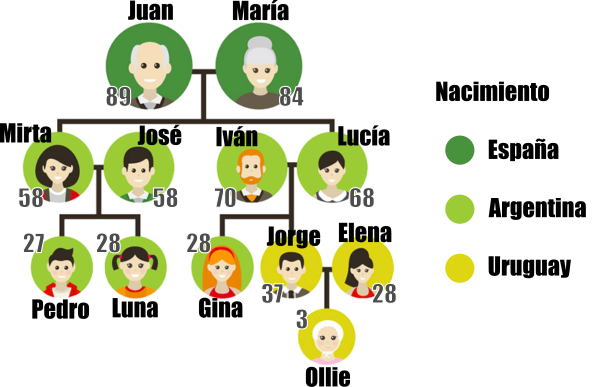
\includegraphics[height=5cm]{familia.png}
	%\end{center}
\end{enumerate}
\vspace{20pt} 
 \textbf{RESPUESTAS}\begin{enumerate}\exercise\begin{enumerate} [label=(\alph*)]		\item Función informativa, es proposición. El valor de verdad dependerá del día.
		\item Función exclamativa, no es una proposición. Notar que gritar "Me acabo de lastimar" sí sería es una proposición.
		\item Función informativa, es proposición. El valor de verdad depende de la persona que lo lea.
		\item Función imperativa, no es proposición.
		\item Función interrogativa, no es proposición.
		\item Función informativa, es proposición. Es falsa.
		\item Función informativa, es proposición. La proposición es verdadera pero tiene detalles discutibles. Para afirmar que para alguna persona es falsa deberiamos pensar en una persona que estudie continuamente pero que no aprenda cosas nuevas.
		\item Función informativa, es proposición. Aunque sean simbolos matemáticos, esta proposición se puede leer como "El número $x$ es seis y el número $x$ sumado a 4 es igual a 10". Lo que hace que esto sea una proposición es que estamos afirmando las igualdades, que el número es igual a 6 y que sumado a 4 es igual a 10. La proposición es V.
		\item No es proposición. Se puede leer como "El número $x$ más 4" y no se afirma nada al respecto. Es similar al inciso de "En las aulas de la UNQ".
		\item Función afirmativa, es una proposición. Para averiguar su valor de verdad debemos buscar las raíces de la parábola, es decir, $x^2-4=0$. Mediante la fórmula de Bhaskara (la resolvente cuadrática) podemos obtener que $x=2$ o $x=-2$. $2$ y $-2$ son números reales. Por lo que la proposición es falsa. 
\end{enumerate}\exercise\begin{enumerate} [label=(\alph*)]		\item $p \land q$ con $p$:"\textit{La manzana es una fruta}" y $q$:"\textit{La lechuga una verdura}". Un equivalente es $q \land p$:"\textit{La lechuga es una verdura y la manzana es una fruta}".
		\item $\neg p$ con $p$:"\textit{Está lloviendo}".
		\item $p\then q$ con $p$:"\textit{Estás en la estación Bernal}" y $q$:"\textit{Estás cerca de la UNQ}". Un equivalente es $\neg q \then \neg p$: "\textit{Si no estás cerca de la UNQ, no estás en la estación de Bernal}".
		\item $\neg p \land q$ con $p$:"\textit{Es buen deportista}" y $q$:"\textit{Sus notas son excelentes}". Un equivalente es $q \land \neg p$:"\textit{Sus notas son excelentes pero no es buen deportista}". Notar que linguísticamente las frases son distintas porque se le da distinta importancia relevancia al orden de las proposiciones, en la primera se rescata que es buen estudiante, en la segunda se condena que es mal deportista. En este caso la lógica no logra mostrar estas diferencias linguísticas. \href{https://youtu.be/HXzyX5XGPp8?t=503}{Resolución por Tu Profe en Linea}.
		\item $p \lor (q \land r)$ con $p$:"\textit{El caballo está galopando}", $q$:"\textit{El caballo de detuvo}" y $r$:"\textit{El caballo relinchó}". \href{https://youtu.be/TgwraosKUuY?t=70}{Resolución por Christian Omar Arias López}.
		\item $p\eq q$ con $p$:"\textit{En la UNQ hay wi-fi}" y $q$:"\textit{Hay luz}". Un equivalente es $(p \then q) \land (q \then p)$:"\textit{Si en la UNQ hay wi-fi, hay luz. Si hay luz, en la UNQ hay wi-fi}".
		\item $p \xor q$ con $p$:"\textit{Mañana lloverá}" y $q$:"\textit{Mañana estará soleado}". Un equivalente es $(p \land \neg q) \land (\neg p \land q)$:"\textit{Mañana lloverá y no estará soleado, o bien, mañana estará soleado y no lloverá}". 
		\item $p \lor q \lor r$ con $p$:"\textit{La materia se aprueba promocionando los parciales}", $q$:"\textit{La materia se aprueba aprobando el final}" y $r$:"\textit{La materia se aprueba dando exitosamente el exámen libre}". También se acepta $p \lor q \lor r \then s$ con el diccionario $p$:"\textit{Promociono los parciales}", $q$:"\textit{Apruebo el final}", $r$:"\textit{Doy exitosamente el exámen libre}" y $s$:"\textit{Apruebo la materia}". Esta simbología captura mejor la situación, pero por otro lado tuvimos que llevarla a la primera persona (yo) y podria haber sido cualquier estudiante. Para mejorar esto se puede utilizar lógica de predicados, que se verá al final de la unidad. Dejo la respuesta para que se revise más adelante. $\forall x: p(x) \lor q(x) \lor r(x) \then s(x)$ con el diccionario $p(x)$:"$x$ \textit{promociona los parciales}", $q(x)$:"$x$ \textit{aprueba el final}", $r(x)$:"$x$ \textit{da exitosamente el exámen libre}" y $s(x)$:"$x$ \textit{aprueba la materia}".
		\item $(q\then \neg p)  \land  (r\then \neg p)$ con $p$:"\textit{El pan levará}", $q$:"\textit{Le pones mucha sal}" y $r$:"\textit{Lo dejas en un lugar frío}". Un equivalente es $(q \lor r) \then \neg p$:"\textit{Si le pones mucha sal o lo dejas en un lugar frío, el pan no levará}".
		\item $( p\then q ) \land ( r\then \neg q )$ con $p$:"\textit{Te tomas el 324}", $q$:"\textit{Te deja cerca de la UNQ}" y $p$:"\textit{Te tomás el 65}".  
\end{enumerate}\exercise\begin{enumerate} [label=(\alph*)]		\item Contingencia. \href{https://www.wolframalpha.com/input?i=%28not+p+or+q%29+and+not+q}{Resolución}.
		\item Contradicción. \href{https://www.wolframalpha.com/input?i=truth+table+of%3A+p+and+not+p}{Resolución}.
		\item Contingencia.\href{https://www.wolframalpha.com/input?i=p+and+r+or++q}{Resolución, ver solo donde $r$ es F}.
		\item Contingencia. \href{https://www.wolframalpha.com/input?i=%28p+%3D%3E+q%29+%3D%3E+r}{Resolución}.
		\item Contingencia. \href{https://www.wolframalpha.com/input?i=p+%3C%3D%3E+%28q+xor++r%29}{Resolución}.
		\item Contingencia. \href{https://www.wolframalpha.com/input?i=%28p+nand+q%29+nor+r}{Resolución}
		\item Es tautología. \href{https://youtu.be/k-amMQR3oMc}{Resolución por ProfeGuille}.
\end{enumerate}\exercise\begin{enumerate} [label=(\alph*)]		\item La \href{https://www.wolframalpha.com/input?i=truth+table%3A+not+%28not+p%29+%3C%3D%3E+p}{tabla de verdad} revelea que es una tautología. Por lo tanto, son equivalentes. Esta regla de equivalencia se llama Doble Negación.
		\item La \href{https://www.wolframalpha.com/input?i=%28p+%3D%3E+q%29+%3C%3D%3E+not+q+%3D%3E+not+p}{tabla de verdad} revela que es una tautología. Por lo tanto, son equivalentes. Esta regla de equivalencia se llama Definición de la Implicación.
		\item La \href{https://www.wolframalpha.com/input?i=%28p+%3D%3E+q%29+%3C%3D%3E+%28not+p+%3D%3E+not+q%29}{tabla de verdad} revela que es una contingencia. Por lo tanto, NO son equivalentes.
		\item La \href{https://www.wolframalpha.com/input?i=%28p+and+%28p+or++q%29%29+%3C%3D%3E++p}{tabla de verdad} revela que es una tautología. Esta regla de equivalencia se llama Absorción Total.
		\item La \href{https://www.wolframalpha.com/input?i=%28p+%3D%3E+q%29+%3C%3D%3E+%28%28p+and+not+q%29+%3D%3E+r%29}{tabla de verdad (ver dónde r es F)} revela que es una tautología. Por lo tanto, son equivalentes. Esta regla de equivalencia se llama Reducción al absurdo.
		\item La \href{https://www.wolframalpha.com/input?i=%28%28p+and+q%29+%3D%3E+r%29%3C%3D%3E+%28p+%3D%3E+%28q+%3D%3Er%29%29}{tabla de verdad} revela que es una tautología. Por lo tanto, son equivalentes. Esta regla de equivalencia se llama Exportación.
		\item La \href{https://www.wolframalpha.com/input?i=%28%28p+or+q+%29+%3D%3E++r%29+%3C%3D%3E+%28+%28p+%3D%3E+r%29+and+%28q+%3D%3E+r%29+%29}{tabla de verdad} revela que es una tautología. Por lo tanto, son equivalentes. Esta regla de equivalencia se llama Demostración por casos.
\end{enumerate}\exercise\begin{enumerate} [label=(\alph*)]		\item La expresion más simple es $q$. \href{https://youtu.be/BOydu7cpv70}{Resolución por Tu Profe en Linea}.
		\item $\neg p \land q$. \href{https://youtu.be/p005yi28rgk?t=737}{Resolución por ProfesorTriquero}.
		\item Puede ser $q \then p$, o bien $p \lor \neg q$. \href{https://youtu.be/p005yi28rgk?t=995}{Resolución por ProfesorTriquero}.
		\item Es equivalente a $T_0$ (es una tautología). \href{https://youtu.be/BOydu7cpv70?t=586}{Resolución por Tu Profe en Linea}.
		\item La expresión mas simple es $q$. \href{https://youtu.be/KyIdCTWZuJ8}{Resolución por ProfeGuille}.
		\item $p \land q$. \href{https://youtu.be/shOOoVRqKcA}{Resolución por ProfeGuille}.
\end{enumerate}\exercise\begin{enumerate} [label=(\alph*)]		\item DNF: $(p\land \neg q) \lor  (\neg p\land q)$ \\ CNF: $(p\lor q) \land  (\neg p\lor \neg q)$
		\item DNF: $(p\land \neg q)$  \\ CNF: $(\neg p\lor \neg q) \land  (p\lor q) \land  (p\lor \neg q)$
		\item DNF: $(p\land q\land r) \lor  (\neg p\land q\land r) \lor  (\neg p\land q\land \neg r) \lor  (\neg p\land \neg q\land r) \lor  (\neg p\land \neg q\land \neg r)$  \\ CNF: $(\neg p\lor \neg q\lor r) \land  (\neg p\lor q\lor \neg r) \land  (\neg p\lor q\lor r)$
\end{enumerate}\exercise\begin{enumerate} [label=(\alph*)]		\item Es tautología, por lo que es una regla de inferencia. Se la llama \textit{Simplificación}. Ver la \href{https://www.wolframalpha.com/input?i=%28p+and+q%29+%3D%3E+p}{tabla de verdad}.
		\item Es contingencia, no es regla de inferencia. Ver la \href{https://www.wolframalpha.com/input?i=%28p+or+q%29+%3D%3E+q}{tabla de verdad}.
		\item Contingencia.
		\item Es tautología, por lo que es una regla de inferencia que no tiene nombre. \href{https://youtu.be/NZSuHeymu4M?t=382}{Resolución por Tu Profe en Linea}.
		\item Es tautología, por lo que es una regla de inferencia. Se la llama \textit{Elimiaciónn del bicondicional}. Ver la \href{https://www.wolframalpha.com/input?i=%28p%3C%3D%3Eq%29+%3D%3E+%28p%3D%3Eq%29}{tabla de verdad}.
		\item Es contingencia, no es regla de inferencia. \href{https://youtu.be/NZSuHeymu4M?t=829}{Resolución por Tu Profe en Linea}.
\end{enumerate}\exercise\begin{enumerate} [label=(\alph*)]		\item \DReasoning{$\neg p\then p$}{$\neg \neg p \lor p$ ~~~(def. $\then$); $p \lor p$ ~~~(doble $\neg$)}{$p$ ~~~(idempotencia)}
		\item \Reasoning{$p\then q$ ; $\neg q$}{$\neg p$ ~~~(modus tollens)}
		\item \DReasoning{$p\then q$ ; $q\then r$ ; $p$}{$p \then r$ ~~~(tran. del $\then$)}{$r$ ~~~(modus ponens)}
		\item \DReasoning{$\neg p$}{$\neg p \lor \neg q$ ~~~(adición)}{$\neg (p\land q)$ ~~~(De Morgan)}
		\item \DReasoning{$p\then r$ ; $q\then r$ ; $r\then s\land t$ ; $p\lor q$}{$r$ ~~~(elim. disy.);$s \land t$ ~~~(modus ponens)}{$s$ ~~~(simplificación)}
		\item Aplicamos exportación: \\ \DReasoning{$p\then q$ ; $q\land r\then s$; $p$; $r$}{$q$ ~~~(modus ponens)}{$s$ ~~~(conj. y mod. pon.)}
		\item \DReasoning{$p\then  q$ ; $q\eq r$ ; $\neg r$}{$q \then r$ ~~~(elim. $\eq$); $\neg q$ ~~~(mod. tollens)}{$\neg p$ ~~~(mod. tollens)}
		\item \DReasoning{$p \then q$ ; $p \lor s$ ; $\neg q$}{$\neg p$ ~~~(mod. toll.)}{$s$ ~~~(mod. toll. pon.)}
\end{enumerate}\exercise\begin{enumerate} [label=(\alph*)]		\item Razonamiento válido. Usamos $m$:"\textit{es martes}", $l$:"\textit{llueve}", $f$:"\textit{hace frio}". Por lo que el razonamiento será \\ \DReasoning{$m \then l \land f$; $m$}{$l \land f$ ~~~(mod. pon.)}{$f$ ~~~(simpl.)}
		\item Razonamiento válido. Utilizando $l$:"\textit{el ladron tenía llave}", $v$:"\textit{el ladron entró por la ventana}" y $p$:"\textit{el ladron pisoteó las macetas}", se demuestra: \\ \DReasoning{$l \lor v$; $v \then p$; $\neg p$}{$\neg v$ ~~~(mod. tollens)}{$l$ ~~~(mod. toll. ponens)} \\  \href{https://youtu.be/DD5EleyOl-0?t=74}{Planteo por Maria Alicia Piñeiro}.
		\item Razonamiento válido. Utilizamos los números enteros $x,y \in \mathbb{Z}$: \\ \DReasoning{$x$ es impar; $y$ es impar}{$x=2k+1$ con $k \in \mathbb{Z}$; $y=2m+1$ con $m \in \mathbb{Z}$;$x.y=(2k+1).(2m+1)=2(2km+k+m)+1$ con $(2km+k+m) \in \mathbb{Z}$}{$x.y$ es impar}
		\item Razonamiento inválido. Contraejemplo: $2+4=6$. $2$ y $4$ son pares, pero $6$ no es impar.
		\item Razonamiento válido. Demostraremos el contrarrecíproco: "\textit{Si un número entero no es impar, el cuadrado de dicho número no es impar}". Utilizamos el numero entero $n \in \mathbb{Z}$: \\ \DReasoning{$n$ no es impar}{$n$ es par; $n=2k$ con $k \in \mathbb{Z}$;$n^2=(2k).(2k)=2(2.k.k)$ con $(2.k.k) \in \mathbb{Z}$;$n^2$ es par}{$n^2$ no es impar}
		\item Razonamiento válido. Utilizamos el numero entero $n \in \mathbb{N}$: \\ \DReasoning{$n$ es múltiplo de $6$}{$n=k.6$ con $k \in \mathbb{N}$; $n=(k.2).3$ con $2k \in \mathbb{N}$;$n=(k.3).2$ con $3k \in \mathbb{N}$}{$n$ es multiplo de 3 y de 2}
		\item Razonamiento válido. \\ \DReasoning{$x<y$}{$y<y+1$ ~~~(prop. suma en $\mathbb{R}$); $x<y+1$ ~~~(transit. del $<$); $(x<y+1) \lor ($x=y+1$)$ ~~~(adición)}{$x \leq y+1$}
		\item Razonamiento válido. \\ \DReasoning{$x^2-x-6>0$}{$(x+2)(x-3)>0$ ~~~(factorizo); $(x>3) \lor (x<-2)$ ~~~(prop. desigualdad); $(x>3) \then |x|>3$ ~~~(prop. val. abs.); $(x<-2) \then |x|>2$ ~~~(prop. val. abs.);$(|x|>3) \lor (|x|>2)$   ~~~(dilema constr.); $|x|>3 \then |x|>1$; $|x|>3 \then |x|>1$}{$|x|>1$ ~~~(elim. disy.)}
		\item Razonamiento válido. \\ \DReasoning{$|x| = |y|$}{$(x = |y|) \lor (x = -|y|)$ ~~~(prop. val. abs.); $(x = |y|) \lor (-x = |y|)$ ~~~(opero algebr.); $(x = y) \lor (-x = y) \lor (-x = y) \lor (-(-x) = y)$ ~~~(prop. val. abs.)}{$(y=x) \lor (y=-x)$ ~~~(idempot.)}
		\item Razonamiento válido. \\ \DReasoning{$a.b = 0$}{$(a=0) \lor (b=0)$; $(a=0) \then y=ax+3$ es horizontal; $(b=0) \then y=mx+b$ pasa por $P(0,0)$}{$y=mx+b$ pasa por $P(0,0) \lor y=ax+3$ es horizontal ~~~(dilema construc.)}
\end{enumerate}\exercise\begin{enumerate} [label=(\alph*)]		\item Dado el universo $U = \{x ~|~ x$ es una persona$\}$, y los predicados  $C(x)$:\textit{"la persona $x$ canta"} y  $G(x)$:\textit{"la persona $x$ toca la guitarra"}. Se simboliza $\exists x: C(x) \lor G(x)$ con su negación $\neg \left(\exists x: C(x) \lor G(x)\right) \Eq \forall x: \neg C(x) \land \neg G(x)$. \href{https://youtu.be/rnaCiSpVtP4}{Resolución por MathLogic}.
		\item Dado el universo $U = \mathbb{N}$ y los predicados $P(x)$:\textit{"$x$ es par"} y $N(x)$:\textit{"$x$ es negativo"}. Se simboliza $\forall x: P(x) \lor N(x)$ con su negación $\neg \left(\forall x: P(x) \lor N(x)\right) \Eq \exists x: \neg P(x) \land \neg N(x)$.
		\item ado el universo $U = \{x ~|~ x$ es un automóvil$\}$ y los predicados $P(x)$:\textit{"$x$ es cómodo"} y $Q(x)$:\textit{"$x$ es caro"}. Se simboliza $\forall x: P(x) \then  Q(x)$
		\item Dado el universo $U = \{x ~|~ x$ es una persona$\}$, y los predicados $F(x)$:\textit{"$x$ tiene frío"}  y $M(x)$:\textit{"$x$ toma mate"}. Se simboliza $\exists x: F(x) \eq  M(x)$.
		\item Dado el universo $U = \{x ~|~ x$ es un animal$\}$, y los predicados $P(x)$:\textit{"$x$ es un pájaro"}, $A(x)$:\textit{"$x$ es un anfibio"} y $Z(x):$\textit{"$x$ es un pez"}. Se simboliza \\ \Reasoning{$\forall x: P(x) \then \neg A(x)$; $\forall x: \neg A(x) \then \neg Z(x)$}{$\forall x: P(x) \then Z(x)$} \\ \href{https://youtu.be/M71MEB3TkVw?t=32}{Resolución por MathLogic}.
\end{enumerate}\exercise\begin{enumerate} [label=(\alph*)]		\item Depende del pronóstico del clima de esa semana
		\item Verdadera, ya que $1 < 26 ~~\land~~ 9 < 26 ~~\land~~ 25 < 26$. \href{https://youtu.be/ChfOh0xG7Ok?t=121}{Resolución por Tu Profe en Linea}.
		\item Verdadera, ya que $1 < 26$ (y con eso basta). \href{https://youtu.be/ChfOh0xG7Ok?t=246}{Resolución por Tu Profe en Linea}.
		\item Falso, ya que $5^2-9=25-9=16 \neq 0$. \href{https://youtu.be/ChfOh0xG7Ok?t=385}{Resolución por Tu Profe en Linea}.
		\item Falso, ya que $10 + 3 = 13 \nless 6$. \href{https://youtu.be/ChfOh0xG7Ok?t=506}{Resolución por Tu Profe en Linea}.
		\item La proposición es verdadera ya que $x=-1$ cumple
		\item La proposición es  verdadera ya que $\left(\forall x: x < 5\right)$ es falsa pero $\left( \exists x: x^2 = 4 \right)$ es verdadera en $x=2$
		\item La proposiciòn es falsa ya que para $x=3$ no existe un $y$ que cumpla.
\end{enumerate}\exercise\begin{enumerate} [label=(\alph*)]		\item Razonamiento válido. \\ \DReasoning{$\forall x: P(x)\then  Q(x) \land  R(x)$; $P(a)$}{$P(a)\then  Q(a) \land  R(a)$ ~~~(part. univ. en $a$); $Q(a) \land  R(a)$ ~~~(mod. ponens); $R(a)$ ~~~(simplif.)}{$\exists x: R(x)$ ~~~(general. exist.)}
		\item Razonamiento válido. \href{https://youtu.be/jf1nYwJEZMs?t=591}{Resolución por MathLogic}.
		\item Razonamiento inválido. \href{https://youtu.be/PtjWjkc5txI?t=535}{Resolución por Maria Alicia Piñeiro}.
		\item Razonamiento válido. \\ \DReasoning{$\neg (\forall x: P(x) \then Q(x))$; $\exists x: \neg (P(x) \then Q(x))$}{$\neg (P(a) \then Q(a))$ ~~~(part. exist.); $\neg (\neg P(a) \lor Q(a))$ ~~~(def. $\then$); $P(a) \land \neg Q(a)$ ~~~(De. Morgan); $P(a)$ ~~~(simpl.)}{$\exists x: P(a)$ ~~~(general. exist.)}
		\item Razonamiento válido. \\ \DReasoning{$\neg \exists x: \neg P(x) \land  \neg Q(x)$; $\neg P(a)$}{$\forall x: \neg (\neg P(x) \land \neg Q(x))$ ~~~(neg. cuantif.); $\neg (\neg P(a) \land \neg Q(a))$ ~~~(part. en $a$); $P(a) \lor Q(a)$ ~~~(De Morgan)}{$Q(a)$ ~~~(mod. toll. pon.)} 
		\item Razonamiento válido. \href{https://youtu.be/PtjWjkc5txI}{Resolución por Maria Alicia Piñeiro}.
		\item Razonamiento válido. \href{https://youtu.be/PtjWjkc5txI?t=328}{Ejercicio parecido por Maria Alicia Piñeiro}.
		\item Razonamiento inválido. Se puede demostrar por contraejemplo: asumiendo que todos los dulces tienen carbohidratos y que hay comidas sin carbohidratos y proteínas, aun puede suceder que no todas las comidas tengan carbohidratos o proteínas, como es el caso de la manteca. \href{https://youtu.be/AMDgepP_N_A?t=892}{Ejercicio parecido por Jonathan Castro}.
\end{enumerate}\exercise\begin{enumerate} [label=(\alph*)]		\item Función informativa, es proposición. Podemos indicar si es verdadero en momentos y lugares donde es posible que llueva, mientras que será falsa si en lugares donde no es posible que llueva.
		\item Función interrogativa, no es proposición.
		\item Función afirmativa, es proposición. Se puede leer como "$R_1$ es perpendicular a $R_2$". Para ver si son perpendiculares debemos revisar la relacion entre sus pendientes. Podemos ver que $m_1 = -\frac{1}{m_2}$ se cumple ya que $1 = -\frac{1}{-1}$. Por lo que la proposición es verdadera.
		\item No es una proposición. Se puede leer como "El intervalo que va desde cero a infinito". Pero carece de afirmación, simplemente enuncia un objeto, es similar al inciso x+4.
		\item Función exclamativa, no es proposición. Notar que "Estoy agradecido con vos" sí sería una proposición.
		\item Función informativa, es proposición. El valor de verdad no depende de si llueve o no, depende de si quien lo dice le parece que llueve o no. Si el narrador está engañando será falsa, si realmente cree que sí será verdadera.
		\item No está clara la función pero es exclamativa o imperativa, en cualqueir caso, no es proposición.
		\item Función afirmativa, es una proposición. Puede leerse como "x es igual a 9 y 2 es menor que x y x es menor que 7". La proposición será verdadera.
		\item No es proposición ya que se está enunciando un objeto sin afirmar nada sobre el mismo. Gramaticalmente podemos decir que es una oración sin verbo. Por otra parte, la función del lenguaje no es clara ya que carecemos de contexto. Notar que si esta oración fuese la respuesta a la pregunta "¿En dónde se cursa?", entonces podríamos interpretar que la respuesta es "(Se cursa) en las aulas de la UNQ" y sí sería una proposición.
		\item No es una proposición. Como $x$ no tiene un valor el enunciado no tendrá un valor de verdad. Este tipo de enunciados los veremos al final de la unidad y se llaman esquemas proposicionales, predicados o enunciados abiertos. Notar que si $x$ fuera un número definido pero desconocido para nosotros sí sería una proposicion con valor de verdad definido (aunque desconocido).
		\item Función exclamativa, no es proposición.
		\item Es complicado. Debemos preguntarnos si hay una afirmación en esta frase. Primero deberíamos reformularla para entender si hay un verbo implicito. "Si alguien te regala un caballo, no deberías mirarle los dientes". Aquí se observa que hay una afirmación sobre si deberíamos mirarle los dientes al caballo o no. Esta afirmación sí es una proposición pero puede ser verdadera o falsa. Si nuestra interpretación de la frase es una órden como "Si te regalan un caballo, no le mires los dientes" esta oración no será una proposición, notar que se pierde el verbo \textit{deberías}. El hecho de que no haya una respuesta clara y correcta sobre este ejercicio muestra que la lógica esta limitada a la interpretación previa del lenguaje.
\end{enumerate}\exercise\begin{enumerate} [label=(\alph*)]		\item $p \then q$ con $q$:"\textit{Luis es feliz}" y $p$:"\textit{Luis escribe poemas}". Un equivalente es $\neg p \lor q$: "Luis no escribe poemas o luis es feliz". \href{https://youtu.be/HXzyX5XGPp8?t=374}{Resolución por Tu Profe en Linea}.
		\item $\neg (p \land \neg q)$ con $p$:"\textit{Estudiamos}" y $q$:"\textit{Aprobamos}". Un equivalente es $\neg p \lor q$:"\textit{No estudiamos o aprobamos}". Otro equivalente es $p \then q$:"\textit{Si estudiamos, aprobamos}". \href{https://youtu.be/HXzyX5XGPp8}{Resolución por Tu Profe en Linea}.
		\item $\neg p  \land  \neg q$ con $p$:"\textit{Me gusta la pizza}" y $q$:"\textit{Me gustan las empanadas}". Un equivalente es $p \downarrow  q$, que se lee igual:"\textit{Ni me gusta la pizza, ni me gustan las empanadas}".
		\item $\neg q \land (\neg q\then \neg p)$ con $p$:"\textit{Hoy es jueves}" y $q$:"\textit{Ayer fue miércoles}". Notar que no solo se debe indicar la relación $\neg q\then \neg p$, sino que también debemos afirmar que $\neg q$.
		\item $p \then  ( q  \land  r )$ con $p$:"\textit{Llueve}", $q$:"\textit{Traigo el impermeable}" y $r$:"\textit{Traigo las botas}". Un equivalente es $(p \then q) \land (p \then r )$:"\textit{Si llueve traigo el impermeable y si llueve traigo las botas}".
		\item $( p \then  q )  \land  ( \neg p \then  \neg q )$ con $p$:"\textit{Has amado}" y $p$:"\textit{Sabés lo que se siente amar}". Un equivalente es $p \eq  q$: "\textit{Has amado si y sólo si sabes lo que se siente amar}".
		\item $((p \land q) \lor r) \eq s$ con $p$:"\textit{El anciano ingresó a la cabaña}", $q$:"\textit{El anciano tomó asiento}", $r$:"\textit{El anciano permaneció afuera}" y $s$:"\textit{El anciano regresó de viaje}". \href{https://youtu.be/TgwraosKUuY?t=331}{Resolución por Christian Omar Arias López}.
		\item $\neg p  \land  \neg q$ con $p$:"\textit{Caminamos con prisa}" y $q$:"\textit{Caminamos con pausa}". Un equivalente es $p \downarrow  q$:"\textit{Ni caminamos con prisa ni caminamos con pausa}"
		\item $( p  \land  q  \land  r ) \land ( p  \land  q  \land  r  \then   s \lor  t )$ con $p$:"\textit{Python es un lenguaje de programación interpretado}", $q$:"\textit{Python es un lenguaje de programación  de propósito general}", $r$:"\textit{Python es un lenguaje de programación de alto nivel}", $s$:"\textit{Python resulta útil para procesar datos}" y $t$:"\textit{Python resulta útil para automatizar tareas simples}".
		\item Hay varias simbolizaciones posibles. Por ejemplo, si reformulamos el enunciado para obtener proposiciones: "\textit{Voy rápido sí y solo si voy despacio y sin pausas}" con las proposiciones $p$:"\textit{Voy rápido}", $q$:"\textit{Voy despacio}" y $r$:"\textit{Voy con pausas}" obtenemos en símbolos $p \eq ( q \land \neg r)$.
		\item $(p \xor q) \land ( p \then  q ) \land  ( r \then  ( s \lor  t) )$ con $p$:"\textit{Termino las tareas en la semana}", $q$:"\textit{Tendré el fin de semana libre}", $r$:"\textit{Termino las tareas durante el fin de semana}", $s$:"\textit{Tendría que abastecerme de café}" y $t$:"\textit{Tendría que abastecerme de mate}".
		\item Primero reformulamos el enunciado:"\textit{Si dedico tiempo y atención a la materia, entonces apruebo}". Entonces tenemos la proposición $( q  \land  r ) \then  p$ con $p$:"\textit{Apruebo}", $q$:"\textit{Dedico tiempo a la materia}" y $r$:"\textit{Dedico atención a la materia}".
		\item Una opcion simple es $\neg p  \land  r$ con $p$:"\textit{Calavera chilla}" y $q$:"\textit{Piola se la banca}". Pero podríamos tener $( p\then q )  \land  ( r\then s )$ considerando $p$:"\textit{Alguien es calavera}", $q$:"\textit{Alguien chilla}", $q$:"\textit{Alguien es piola}" y $q$:"\textit{Alguien se la banca}"
		\item $( p  \land  q ) \land ( p  \land  q  \then  r \lor  s )$ con $p$:"\textit{Vine en tren}", $q$:"\textit{Suspendieron el servicio}", $r$:"\textit{Tengo que volver en colectivo}" y $s$:"\textit{Tengo que volver caminando}". Notar que además de enunciar la relacion de implicación entre las proposiciones se debe afirmar que se cumple el antecedente.
		\item $( p  \land  q )  \land  r  \land  s $. $p$:"\textit{En un juego son importantes las mecánicas}", $q$:"\textit{En un juego es importantes la historia}", $r$:"\textit{Las mecánicas mantienen a la persona jugadora activa}" y $s$:"\textit{La historia la mantiene interesada}".
		\item $( q \then  p ) \eq  ( p \lor  \neg q)$ con $p$:"\textit{Los fantasmas se ponen azules}" y $q$:"\textit{El pacman come la fruta}".
\end{enumerate}\exercise\begin{enumerate} [label=(\alph*)]		\item Contingencia. \href{https://www.wolframalpha.com/input?i=p+or++%28not+q+xor++r%29}{Resolución}
		\item Contingencia. \href{https://www.wolframalpha.com/input?i=p+and++q+or++r}{Resolución}.
		\item Contingencia. \href{https://www.wolframalpha.com/input?i=not+%28p+%3D%3E+%28q+and++r%29%29}{Resolución}.
		\item Contradicción. \href{https://www.wolframalpha.com/input?i=not+%28%28p+nor+q%29+%3D%3E+r%29}{Resolución, ver sólo donde $p$ es V}.
		\item Es contradicción. \href{https://youtu.be/n_t1f0xa3D0?t=413}{Resolución por ProfeGuille}.
		\item Es tautología. \href{https://youtu.be/n_t1f0xa3D0?t=643}{Resolución por ProfeGuille}.
		\item Es contradicción. \href{https://youtu.be/rlJmcBGdOoY}{Resolución por ProfeGuille}.
		\item Es contingencia. \href{https://youtu.be/n_t1f0xa3D0?t=40}{Resolución por ProfeGuille}.
\end{enumerate}\exercise\begin{enumerate} [label=(\alph*)]		\item La \href{https://www.wolframalpha.com/input?i=truth+table%3A%28not+p+%3D%3E+p%29+%3C%3D%3E+p}{tabla de verdad} revela que es una tautología. Por lo tanto, son equivalentes. Esta regla de equivalencia no tiene nombre (ni es muy útil). 
		\item La \href{https://www.wolframalpha.com/input?i=%28not+p+or+not+q%29+%3C%3D%3E+%28p+and+q%29}{tabla de verdad} revela que es una contradicción. Por lo tanto, las proposiciones no son equivalentes.
		\item La \href{https://www.wolframalpha.com/input?i=%28p+and+not+q%29+%3C%3D%3E+%28not+p+or+q%29}{tabla de verdad} revela que es una contradicción. Por lo tanto, las proposiciones no son equivalentes. También pueden ver la \href{https://youtu.be/NZSuHeymu4M?t=639}{resolución por Tu Profe en Linea}.
		\item La \href{https://www.wolframalpha.com/input?i=%28p+%3D%3E+%28q+or+r%29%29+%3C%3D%3E+%28%28p+and+r%29+%3D%3E+%5Cneg+q%29}{tabla de verdad} revela que es una contingencia. Por lo tanto, las proposiciones no son equivalentes. Para más detalles ver la \href{https://www.youtube.com/live/-yHPDgU-lfE?feature=share&t=578}{resolución por Julio Profe}.
		\item La \href{https://www.wolframalpha.com/input?i=not+%28%28p+and+q%29+%3D%3E+not+r%29+%3C%3D%3E++%28%28p+and+q%29+or+r%29}{tabla de verdad} revela que es una contingencia. Por lo tanto, no son equivalentes. 
		\item La \href{https://www.wolframalpha.com/input?i=truth+table%3A+%28p+%3D%3E+%28q+and+r+and+s%29%29+%3C%3D%3E+%28%28p+%3D%3E+q%29+and+%28p+%3D%3E+r%29+and+%28p+%3D%3E+s%29%29}{tabla de verdad} revela que es una tautología. Por lo tanto, son equivalentes. Esta regla de equivalencia no tiene nombre.
\end{enumerate}\exercise\begin{enumerate} [label=(\alph*)]		\item Puede ser $q \then p$, o bien $p \lor \neg q$. \href{https://youtu.be/5r8S-wMJq7I}{Resolución por ProfeGuille}.
		\item $\neg p \land q$. \href{https://youtu.be/Ayk4qXcoiOM}{Resolución por ProfeGuille}.
		\item La expresión más simple es $\neg q$. \href{https://youtu.be/BOydu7cpv70?t=884}{Resolución por Tu Profe en Linea}.
		\item Puede ser $q \then p$, o bien $p \lor \neg q$. \href{https://youtu.be/BOydu7cpv70?t=334}{Resolución por Tu Profe en Linea}.
		\item Puede ser $p \then \neg q$, o bien $\neg ( p \land q )$, o también $\neg p \lor \neg q$. \href{https://youtu.be/p005yi28rgk?t=392}{Resolución por ProfesorTriquero}.
		\item La expresión mas simple es $\neg p$. \href{https://youtu.be/UZDME4cZxNc}{Resolución por ProfeGuille}.
		\item La expresión mas simple es $\neg q$. \href{https://youtu.be/DbjwP3w5yTE}{Resolución por ProfeGuille}.
\end{enumerate}\exercise\begin{enumerate} [label=(\alph*)]		\item DNF: $(p\land \neg q)$  \\ CNF: $(\neg p\lor \neg q) \land  (p\lor q) \land  (p\lor \neg q)$
		\item DNF: $(p\land q\land r) \lor  (p\land \neg q\land \neg r) \lor  (\neg p\land q\land \neg r) \lor  (\neg p\land \neg q\land r)$  \\ CNF: $(\neg p\lor \neg q\lor r) \land  (\neg p\lor q\lor \neg r) \land  (p\lor \neg q\lor \neg r) \land  (p\lor q\lor r)$
		\item DNF: $p \land q \land \neg r$ \\ CNF: $(\neg p \lor \neg q \lor \neg r)\land (\neg p \lor q \lor \neg r)\land (\neg p \lor q \lor r)\land (p \lor \neg q \lor \neg r)\land (p \lor \neg q \lor r)\land (p \lor q \lor \neg r)\land (p \lor q \lor r)$
\end{enumerate}\exercise\begin{enumerate} [label=(\alph*)]		\item \DReasoning{$p\then q$ ; $r\land p$ ; $q\eq s$}{$q \then s$ ~~~(elim. $\eq$); $p$ ~~~(simplif.); $q$ ~~~(mod. ponens); $s$ ~~~(mod. ponens)}{$q\land s$ ~~~(conjunción)}
		\item Aplicamos exportación y casos. Caso 1: \\ \DReasoning{$p\then q$ ; $q\lor r\then s$;$p$}{$q$ ~~~(modus ponens); $q \lor r$ ~~~(adición)}{$s$ ~~~(modus ponens)} \\ Caso2: \\ \DReasoning{$p\then q$ ; $q\lor r\then s$;$r$}{$q \lor r$ ~~~(adic. y conmut.)}{$s$ ~~~(modus ponens)}
		\item Aplicamos exportación: \\ \DReasoning{$p\then q$ ; $r\then s$;$p$;$r$}{$q$ ~~~(mod. ponens); $s$ ~~~(mod. ponens)}{$q\land s$ ~~~(conjunción)}
		\item \DReasoning{$p \then q$ ; $s \lor \neg q$ ; $\neg s$}{$\neg q$ ~~~(mod. toll. pon.)}{$\neg p$ ~~~(mod. toll.)}
		\item \DReasoning{$p \land q$ ; $(p \lor r) \then t$}{$p$ ~~~(simpl.); $p \lor r$ ~~~(adición); $t$ ~~~(mod. ponens)}{$p\land t$ ~~~(conjunción)}
		\item Recordar que no hace falta usar todas las premisas: \\ \Reasoning{$p \lor q$ ; $r \lor s$ ; $p \then r$ ; $q \then s ;\neg r$}{$s$ ~~~(m.t.p. premisas 2 y 5)}
		\item \DReasoning{$p \then q$ ; $q \then r$  ; $s \then t$ ; $p \lor  s$}{$p \then r$ ~~~(transit. de $\then$)}{$r\lor t$ ~~~(dilema construc.)}
		\item Por contradicción (asumo $p$): \\ \DReasoning{$p \then q$ ; $(p \land  q) \then r$ ; $\neg(p \land  q)$;$p$}{$q$ ~~~(mod pon.); $(p \land q) \land \neg (p \land q)$ ~~~(conj.)}{$F_0$ ~~~(binarismo excl.)}
		\item \DReasoning{$q \then r$ ; $\neg s \then (t \then u)$ ; $s \lor (q \lor t)$ ; $\neg s$}{$t \then u$ ~~~(mod. pon.); $q \lor t$ ~~~(mod. tol. pon)}{$r\lor u$ ~~~(dilema construc.)}
		\item Demostramos $p \then r$ usando exportación: \\ \DReasoning{$p \lor q \then r$; $r \then p \land s$;$p$}{$p \lor q$ ~~~(adición)}{$r$ ~~~(mod. ponens)} \\ Demostramos $r \then p$ usando exportación: \\ \DReasoning{$p \lor q \then r$; $r \then p \land s$;$r$}{$p \land s$ ~~~(mod. ponens)}{$p$ ~~~(simpl.)} \\ Por lo tanto, $p \eq r$.
\end{enumerate}\exercise\begin{enumerate} [label=(\alph*)]		\item $r$ es F 
		\item $p$ es F y $q$ es V
		\item $p$ es V y $q$ es V
		\item $q$ es F, $r$ es F y $s$ es F
		\item $p$ es V y $q$ es V
		\item $((r \then q) \xor \neg r) \land p$ es F. \href{https://youtu.be/bitBrw1NvNk?t=663}{Resolución por Tu Profe en Linea}.
		\item $((r \land \neg p) \land (q \lor p)) \then r$ es V. \href{https://youtu.be/bitBrw1NvNk?t=793}{Resolución por Tu Profe en Linea}.
		\item $p$ es V, $q$ es F y $r$ es V. \href{https://youtu.be/bitBrw1NvNk}{Resolución por Tu Profe en Linea}.
		\item $p$ es V, $q$ es F, $r$ es V y $s$ es V. \href{https://youtu.be/bitBrw1NvNk?t=140}{Resolución por Tu Profe en Linea}.
		\item $p$ es V, $q$ es V y $t$ es F. \href{https://youtu.be/bitBrw1NvNk?t=273}{Resolución por Tu Profe en Linea}.
		\item $p$ es V, $q$ es F y $r$ es F. \href{https://youtu.be/bitBrw1NvNk?t=465}{Resolución por Tu Profe en Linea}.
		\item $(\neg q \then \neg p) \xor (r \then s)$ es F y $(\neg p \lor q) \land (s \land \neg r)$ es V. \href{https://youtu.be/p005yi28rgk}{Resolución por ProfesorTriquero}.
		\item $p \then q$ es F, $r \xor s$ es V y $(p \lor q) \then (\neg s \xor t)$ es V. \href{https://youtu.be/-VaC5y-rrMI}{Resolución por Tu Profe en Linea}.
\end{enumerate}\exercise\begin{enumerate} [label=(\alph*)]		\item Razonamiento válido. Usamos $m$:"\textit{es martes}", $l$:"\textit{llueve}", $f$:"\textit{hace frio}". Por lo que el razonamiento será \\ \DReasoning{$m \then l \land f$; $\neg l$}{$\neg l \lor \neg f$ ~~~(adición); $\neg (l \land f)$ ~~~(De Morgan)}{$\neg m$ ~~~(mod. tol.)}
		\item Razonamiento válido. Utilizando $b$:"\textit{bajo de peso}", $d$:"\textit{hago dieta}", $g$:"\textit{voy al gimnasio}" y $s$:"\textit{gasto dinero}", se demuestra: \\ \DReasoning{$b \then d \lor g$; $g \then s$; $b; \neg s$}{$d \lor g$ ~~~(mod. pon.); $\neg g$ ~~~(mod. tol.)}{$d$ ~~~(mod. tol. pon.)} \\ \href{https://youtu.be/DD5EleyOl-0?t=255}{Planteo por Maria Alicia Piñeiro}.
		\item Razonamiento válido. \href{https://youtu.be/rEB0nEdSFXo}{Resolución por Maria Alicia Piñeiro}.
		\item Razonamiento válido. \href{https://youtu.be/yAGoR6FUyi8}{Resolución por Aula de Matemática}.
		\item Razonamiento válido. \href{https://youtu.be/yAGoR6FUyi8?t=159}{Resolución por Aula de Matemática}.
		\item Razonamiento válido. \href{https://youtu.be/yAGoR6FUyi8?t=310}{Resolución por Aula de Matemática}.
		\item Razonamiento válido. Demostraremos el contrarrecíproco: "\textit{Si un nùmero no es impar, el resultado de multiplicarlo por 5 y sumarle 3 no será par}": Utilizamos el numero entero $n \in \mathbb{Z}$\\ \DReasoning{$n$ es par}{$n=2k$ con $k\in \mathbb{Z}$; $5n+3=10k+3=2(5k+1)+1$ con $(5k+1) \in \mathbb{Z}$;$5n+3$ es impar}{$5n+3$ no es par}
		\item Razonamiento inválido. Contraejemplo: $3+6=9$. $3$ y $6$ son múltiplos de 3, pero $9$ no es par
		\item Razonamiento inválido. Contraejemplo: $3+6=9$. $3$ es múltiplo de 3 y $6$ es múltiplo de 2, pero $9$ es múltiplo de 3.
		\item Razonamiento inválido. Contraejemplo: $30$ es múltiplo de 10, pero no es múltiplo de 100.
		\item Razonamiento válido. \href{https://youtu.be/wbGe5hIjFUo}{Resolución por Aula de Matemática}.
		\item Razonamiento válido. \href{https://youtu.be/kLjDAzcKWMI}{Resolución por Aula de Matemática}.
\item ---		\item Razonamiento válido. Utilizamos las rectas $R_1$, $R_2$ y $R_3$ a partir de la ecuación $y=mx+b$. \\ \DReasoning{$R_1 \perp  R_2$; $R_2 \perp  R_3$}{$m_2 = -\frac{1}{m_1}$;$m_2 = -\frac{1}{m_3}$; $m_1 = m_3$ ~~~(despeje); $(m_1 = m_3) \land T_0$ ~~~(identidad); $(m_1 = m_3) \land \left[(b_1=b_3) \lor (b_1 \neq b_3)\right]$ ~~~(binar. excl.); $\left[(m_1 = m_3) \land (b_1=b_3)\right] \lor \left[(m_1 = m_3) \land  (b_1 \neq b_3)\right]$ ~~~(distribut.)}{$(R_1 \sim R_3) \lor (R_1 \parallel  R_3)$ ~~~(props. $\sim$ y $\parallel$)}
		\item Razonamiento inválido. Se puede refutar mediante: \\ \DReasoning{$k>2$}{$k^2>4$;$k^2-4>0$; $b^2-4ac=k^2-4$ ~~~(calc. discrim.); $b^2-4ac>0$}{$x^2+k.x+1$ tiene 2 raíces reales} \\ También se puede buscar un contraejemplo: $k=3$ y $x^2+3.x+1$ tiene las raíces reales $x_1=\frac{-3-\sqrt{5}}{2}$ y $x_2=\frac{-3+\sqrt{5}}{2}$.
		\item Razonamiento válido. \\ \DReasoning{$a.b < 0$;$|a|>b>0$}{$(a>0 \land b<0) \lor (a<0 \land b>0)$ ~~~(condición desigualdad); $b>0$ ~~~(simplif.); $a>0$ ~~~(distr., ident. y simplif.); $-4a>0$ ~~~(calc. discrim.)}{$x^2+a$ tiene dos raíces reales.}
\end{enumerate}\exercise\begin{enumerate} [label=(\alph*)]		\item Dado el universo $U = \{x ~|~ x$ es un automóvil$\}$ y los predicados $V(x)$:\textit{"$x$ es veloz"}, $C(x)$:\textit{"$x$ es cómodo"}. Se simboliza $\exists x: V(x) \land  Q(x)$
		\item Dado el universo $U = \mathbb{Z}$ y los predicados $P(x)$:\textit{"$x$ es múltiplo de 5"} y $Q(x)$:\textit{"$x$ es impar"}. Se simboliza $\neg \left(\forall x: P(x) \then  Q(x) \right)$
		\item Dado el universo $U = \mathbb{N}$ y los predicados  $P(x)$:\textit{"$x$ es múltiplo de 2"} y $Q(x)$:\textit{"$x$ es múltiplo de 3"}. Se simboliza $\exists x: P(x) \land  \neg Q(x)$
		\item Dado el universo $U = \{x ~|~ x$ es una taza de mi cocina $\}$ y los predicados $P(x)$: \textit{"mi abuela me regaló la taza $x$"} y $Q(x)$: \textit{"la taza $x$ es de porcelana"}. Se simboliza $\forall x: P(x) \then Q(x)$, $\exists x: P(x) \land Q(x)$, $\forall x: P(x) \land Q(x)$. \href{https://youtu.be/aI-G5V-IGfA}{Resolución por Maria Alicia Piñeiro}.
		\item Dado el universo $U = \{x ~|~ x$ es una cosa $\}$ y los predicados $F(x)$:\textit{"$x$ es fácil"}, $A(x)$:\textit{"$x$ es agradable"}, $E(y)$:\textit{"$y$ estudiará"} y la constante $m=$Marta. Se simboliza \\  \Reasoning{$\left(\forall x: F(x) \land A(x) \right) \then \neg E(m)$;$\neg \left( \exists x: \neg A(x) \right)$;$\forall x: F(x)$}{$\neg E(m)$}. \\\href{https://youtu.be/M71MEB3TkVw?t=736}{Resolución por MathLogic}.
		\item \href{https://youtu.be/M71MEB3TkVw?t=1191}{Resolución por MathLogic}.
		\item Dado el universo $U = \{x ~|~ x$ es una persona$\}$, y los predicados $D(x)$:\textit{"$x$ duerme"}, $S(x)$:\textit{"$x$ tiene sueño"}, $J(x)$:\textit{"$x$ es joven"}, $A(x)$:\textit{"$x$ es arquitecto"}, $R(x)$:\textit{"$x$ escucha la radio"} y $C(x)$:\textit{"$x$ usa la computadora"}. Se simboliza $\neg D(Ana)$, $\forall x:S(x) \then  D(x)$, $\exists x: J(x) \land  S(x)$, $\forall x: A(x) \land  \neg S(x) \then  R(x)$, $\forall x: J(x) \then  S(x) \lor  C(x) $, $A(Marcos) \land  C(Marcos)$, $\neg \left(\exists x: R(x) \land  C(x) \right)$ y finalmente $\exists x: \neg A(x) \land  R(x) \land  S(x) $.
\end{enumerate}\exercise\begin{enumerate} [label=(\alph*)]		\item Falso. \href{https://youtu.be/ChfOh0xG7Ok?t=305}{Resolución por Tu Profe en Linea}.
		\item Verdadero, ya que $3^2-9=9-9=0$. \href{https://youtu.be/ChfOh0xG7Ok?t=460}{Resolución por Tu Profe en Linea}.
		\item Verdadero, ya que $2 + 3 = 5 \nless 6$. \href{https://youtu.be/ChfOh0xG7Ok?t=557}{Resolución por Tu Profe en Linea}.
		\item La proposición es falsa, ya que $20 \in \mathbb{Z} \land 20-5 = 13 \nless 8$. \href{https://youtu.be/rnaCiSpVtP4?t=303}{Resolución por MathLogic}.
		\item Como $\left(\forall x: P(x) \then  Q(x) \right)$ es falsa, toda la proposición es falsa
		\item La proposiciòn es falsa. $\left(\forall x \exists y: x+y = 2 \right)$ es falsa ya que para $x=3$ no existe $y$ que cumpla, $\neg \left(\forall x \exists y: x+y = 4 \right)$ es falsa ya que para $x=1$ tenemos $y=3$, para $x=2$ tenemos $y=2$, para $x=3$ tenemos $y=1$ y finalmente $\left(\forall x \forall y: x+y \geq  4 \right)$ es falsa ya que para $x=2$ e $y=1$ no se cumple. 
		\item La proposición es verdadera. Dado un $x$ genérico puedo elegir $y=1-x$ que cumple la proposición. 
		\item La proposición es falsa. Para un determinado $y$ debo elegir un $x$ que cumpla $x^2 < y < x$, es decir, $x^2 < x$. Ningún $x \in \mathbb{N}$ cumple esa condición.
		\item La proposición es verdadera. Como $x \leq y < y+2$, si $x$ cumple el antecedente $x \leq  y$, seguro cumple el consecuente $x < y+2$. 
		\item Verdadero, si elegimos $z=\displaystyle\frac{x+y}{2}$ (el promedio), cumplirá la condición. F, por las propiedades de la igualdad, que se cumplen para todos los número reales.
		\item Falso, por las propiedades de la igualdad, que se cumplen para todos los número reales.
		\item Verdadero. $\left(\exists x: P(x)\right)$ es verdadero y se pueden probar las 9 combinaciones de valores de $y$ y $z$ para demostrar  que $\left(\forall y ~\forall z: P(y) \land P(z) \then y=z \right)$ también.
		\item Verdadero ya que sólo $P(1)$ es verdadero
		\item Falso ya que $P(2)$ y $P(3)$ son verdaderas
\end{enumerate}\exercise\begin{enumerate} [label=(\alph*)]		\item Razonamiento válido. \\ \DReasoning{$\neg \exists x: \neg P(x) \land  Q(x)$; $\forall x:  P(x) \then  R(x)$; $Q(a)$}{$\forall x: \neg( \neg P(x) \land Q(x))$ ~~~(neg. cuantif.); $\neg( \neg P(a) \land Q(a))$ ~~~(part. en $a$); $P(a) \lor \neg Q(a)$ ~~~(De Morgan); $P(a)$ ~~~(mod. toll. pon.); $P(a) \then  R(a)$ ~~~(part. en $a$)}{$R(a)$ ~~~(mod. pon.)}
		\item \DReasoning{$\forall x: P(x) \then  Q(x) \land  R(x)$; $\forall x: R(x) \lor  S(x) \then  T(x)$; $P(a)$}{$P(a) \then  Q(a) \land  R(a)$ ~~~(part. en $a$); $Q(a) \land  R(a)$ ~~~(mod. pon.); $R(a)$ ~~~(simplif.); $R(a) \lor  S(a)$ ~~~(adición); $R(a) \lor  S(a) \then  T(a)$ ~~~(part. en $a$)}{$T(a)$ ~~~(mod. pon.)}
		\item \DReasoning{$\forall x\forall y\forall z:  P(x,y)\land P(y,x) \then  (P(x,z)\eq P(y,z)) $; $P(a,b)$; $P(b,c)$; $P(b,a)$}{$P(a,b)\land P(b,a) \then  (P(a,c)\eq P(b,c))$ ~~~(part. $x=a$, $y=b$, $z=c$);$P(a,c)\eq P(b,c)$ ~~~(mod. ponens)}{$P(a,c)$ ~~~(mod. pon. del $\eq$)}
		\item Razonamiento válido. \href{https://youtu.be/DD5EleyOl-0?t=996}{Resolución por MathLogic}.
		\item Razonamiento válido. \href{https://youtu.be/0Dcg9nDzkys?t=1194}{Resolución por Maria Alicia Piñeiro}.
		\item Razonamiento válido. \href{https://youtu.be/AMDgepP_N_A}{Resolución por Jonathan Castro}.
		\item Razonamiento inválido. Se puede demostrar por contraejemplo, definiendo un universo de sillones a elección. \href{https://youtu.be/kszEIGQ1XOA}{Resolución por Maria Alicia Piñeiro}.
		\item Razonamiento válido. Se puede demostrar por contraejemplo, definiendo un universo de sillones a elección. \href{https://youtu.be/kszEIGQ1XOA?t=285}{Resolución por Maria Alicia Piñeiro}.
		\item Razonamiento válido. \href{https://youtu.be/6QGZCc6QbVE}{Resolución por Maria Alicia Piñeiro} y su \href{https://youtu.be/C-BJgBFUIPA}{continuación}.
\end{enumerate}\exercise\begin{enumerate} [label=(\alph*)]		\item Por ejemplo, 10 y 12 para que sea V, y -6 y -7 para que sea F. \href{https://youtu.be/DLsV_L097gE?t=687}{Resolución por MathLogic}.
		\item Las expresiones no son equivalentes. \href{https://youtu.be/WC7P8FMIHFw}{Resolución por Maria Alicia Piñeiro}.
		\item Algunos ejemplos son $P(1)$, $P(2)$, $P(3)$, $\forall x: 2x+1>2$, $P(1) \land P(2)$, $\exists x: 2x+1 \leq 2$. \href{https://youtu.be/rnaCiSpVtP4?t=633}{Resolución por MathLogic}.
\end{enumerate}\exercise\begin{enumerate} [label=(\alph*)]		\item Historicamente se ha utilizado la corriente electrica para para tener dichos estados. Cuando los transistores tienen un voltaje \textit{alto} se activa el paso de corriente emulando el estado V, mientras que si tienen un voltaje \textit{bajo} no pasará corriente y estarán en estado F. Sin embargo para establecer los dos estados se puede utilizar cualquier tipo de corriente, Steve Mould utilizó \href{https://youtu.be/IxXaizglscw}{agua} y varias personas han experimentado con dominos, entre ellos, \href{https://youtu.be/SudixyugiX4}{Neil Fraser}, \href{https://youtu.be/OpLU__bhu2w}{Stand-up Maths} y \href{https://youtu.be/lNuPy-r1GuQ}{Numberphile}.  
		\item Una opción es utilizar tres corrientes: baja, uno mediana y uno alta. La dificultad a partir de allí es armar maquinas físicas que logren representar las compuertas lógicas a partir de dichos voltajes. Análogamente cualquier cosa que represente una corriente (como agua o dominós) podría ser empleada. 
		\item La dificultad principal para representar los estados lógicos es pasar de procesos físicos analógicos, con posibilidad de tener infinitos valores, a valores digitales con dos estados bien definidos. 
		\item El álgebra de Boole es un sistema matemático para representar variables lógicas. Para constituir el sistema se definen operaciones complemento, suma, producto, etc), valores que pueden tomar las variables (0,1) y otras notaciones y reglas que permiten modelar circuitos lógicos.
		\item Negación $\neg p$ se escribe $\bar{p}$, conjunción $p\land q$ es producto $p.q$ y disyunción $p \lor q$ es suma $p+q$. Estas operaciones se definen para ser utilizadas con los valores $0$ y $1$ a partir de reglas internas, por ejemplo los casos que definen a la siyunción son $0+0=0$, $1+0=1$, $0+1=1$, $1+1=1$, que son análogos a la tabla de verdad.
		\item A la DNF se le suele llamar \textit{suma de productos} y a la CNF \textit{producto de sumas}.
\item ---\item ---\item ---\end{enumerate}\end{enumerate}\end{document}